\documentclass[12pt%
%,draft%
,xcolor=table
,aspectratio=169%
]{beamer}
%
\usepackage{fontspec}
\defaultfontfeatures{Ligatures=TeX}
%\setsansfont{Liberation Sans}
\usepackage{polyglossia}
\setdefaultlanguage{ngerman}
% Alternative template for talks of the Freie Universität Berlin.
% Created by Leonard R. König, <leonard.koenig@fu-berlin.de> following the
% guidelines on www.fu-berlin.de/cd
%
% (c) Leonard König, CC BY 4.0
%
% This template was written against UTF-8 capable LaTeX engines, specifically
% LuaLaTeX.

% Trying to get rather close to the ppt/odp template:
%  http://www.fu-berlin.de/sites/cd/downloads_container/PowerPoint_Praesentation_Anleitung.pdf

%%% font styles
\setbeamerfont{frametitle}{series=\bfseries}
\setbeamerfont{footline}{series=\bfseries}
\setbeamerfont{headline}{series=\bfseries}
\setbeamerfont{alerted text}{series=\bfseries}
%%%

% colordefs
\definecolor{fu_darkblue}{RGB}{0,51,102}
\definecolor{fu_seablue}{RGB}{0,102,204}
\definecolor{fu_lightblue}{RGB}{204,214,224}
\definecolor{fu_green}{RGB}{153,204,0}
\definecolor{fu_lightgrey}{RGB}{128,128,128}
\definecolor{fu_grey}{RGB}{95,95,95}
%
\definecolor{fu_red}{RGB}{204, 0, 0} % red text (used by \alert)
%%% end colordefs

%%% colors
\setbeamercolor*{title}{fg=fu_darkblue}
\setbeamercolor*{subtitle}{fg=fu_seablue}
\setbeamercolor*{frametitle}{fg=fu_darkblue}
\setbeamercolor*{footline}{fg=fu_grey,bg=fu_lightblue}
\setbeamercolor*{headline}{fg=fu_grey}

\setbeamercolor*{normal text}{fg=black}
\setbeamercolor*{alerted text}{fg=fu_red}
\setbeamercolor*{example text}{fg=fu_green}
\setbeamercolor*{structure}{fg=fu_darkblue}

\setbeamercolor*{block title}{fg=white,bg=black!50}
\setbeamercolor*{block title alerted}{fg=white,bg=black!50}
\setbeamercolor*{block title example}{fg=white,bg=black!50}

\setbeamercolor*{block body}{bg=black!10}
\setbeamercolor*{block body alerted}{bg=black!10}
\setbeamercolor*{block body example}{bg=black!10}

\setbeamercolor{bibliography entry author}{fg=fu_darkblue}

\setbeamercolor{item}{fg=fu_darkblue}
\setbeamercolor{navigation symbols}{fg=fu_lightgrey,bg=fu_grey}
%%% end colors

%%% title page
% Display logo (if exists) and right next to it, put our title + subtitle
\defbeamertemplate*{title page}{fu_titlepage}
{%
	\hskip .3\textheight
	\begin{minipage}[.4\textheight]{\textwidth}
		\begin{minipage}[.4\textheight]{0.25\textwidth}
			\inserttitlegraphic
		\end{minipage}%
		\begin{minipage}[.4\textheight]{0.75\textwidth}
			\begin{beamercolorbox}{title}
				\usebeamerfont{title}\inserttitle\par%
			\end{beamercolorbox}
			\vfill
			\ifx\insertsubtitle
				\@empty%
			\else
				\begin{beamercolorbox}{subtitle}
					\usebeamerfont{subtitle}\insertsubtitle\par
				\end{beamercolorbox}
			\fi
		\end{minipage}
	\end{minipage}%
	\hskip .3\textheight
}
%%% end title page

%%% headline
% display title, author and institute on the left;
% logo on the right.
\newcommand{\headlinetext}
{%
	\inserttitle\\[0.3em]%
	\insertauthor, %
	\insertshortinstitute
}
\newlength{\headlinewidth}
\setlength{\headlinewidth}{\paperwidth}
\addtolength{\headlinewidth}{-2\marginparsep}
\setbeamertemplate{headline}
{%
	\begin{beamercolorbox}[wd=\paperwidth]{headline}%
		\vskip5pt
		{\hspace*{\marginparsep}}%
		\parbox{.5\headlinewidth}
		{%
			\usebeamertemplate{title in head/foot}%
			\headlinetext%
		}%
		\begin{minipage}{.5\headlinewidth}%
			\hfill\usebeamertemplate*{logo}
		\end{minipage}%
		{\hspace*{\marginparsep}}%
	\end{beamercolorbox}%
}
%%% end headline

%%% footline
% title + date on the left, frame number on the right
\newcommand{\footlinetext}
{%
	\usebeamerfont{shorttitle}\insertshorttitle, %
	\usebeamerfont{shortdate}\insertshortdate
}
\setbeamertemplate{footline}
{%
	\begin{beamercolorbox}{footline}
		\vskip2pt
		\hspace{\marginparsep}%
		\footlinetext\hfill%
		\insertframenumber%
		\hspace{\marginparsep}
		\vskip2pt
	\end{beamercolorbox}%
}
%%% end footline

% don't use default templates for sidebars
\setbeamertemplate{sidebar right}{}
\setbeamertemplate{sidebar left}{}
\setbeamertemplate{title page}[fu_titlepage]
\usepackage{amsmath}
\usepackage{amsfonts}
\usepackage{amssymb}
\usepackage{graphicx}
\usepackage{algorithm}
\usepackage[noend]{algpseudocode}
%\usepackage{algorithmic}
\usepackage{tikz}
\usetikzlibrary{arrows,shapes,automata,petri,positioning,calc}
\usepackage{graphicx}
\usepackage{subfig}
\usepackage{pgfplots}
\usepackage{ stmaryrd }
\usepackage[normalem]{ulem}
\usepackage{circuitikz}
\usepackage{bohr}
\usepackage{csquotes}

\setbeamercolor{block title}{use=structure,fg=white,bg=structure.fg!75!black}
\setbeamercolor{block body}{parent=normal text,use=block title,bg=block title.bg!10!bg}


\usepackage{expl3}

\ExplSyntaxOn
\cs_new:Npn \displayasdecimal#1 {(#1) \sb {10}}
\cs_new:Npn \displayasoctal #1 {(\int_to_oct:n{#1}) \sb 8}
\cs_new:Npn \displayasbinary #1 {(\int_to_bin:n{#1}) \sb 2}
\ExplSyntaxOff

\newcounter{divline}
\def\rlwd{.5pt} \def\rlht{\dimexpr\dp\strutbox+\ht\strutbox} \def\rldp{.75ex}
\newcommand\mydiv[3][\relax]{%
  \ifx\relax#1\stepcounter{divline}\else\setcounter{divline}{#1}\fi%
  \mbox{}\hspace{\thedivline\dimexpr1ex}#2~\setbox0=\hbox{~$#3$}%
  \dumbstackengine{-\rlwd}{\rule[-\rldp]{\rlwd}{\rlht}~#3}{\rule{\dimexpr4pt+\wd0}{\rlwd}}%
}
\def\remainder#1{\stepcounter{divline}%
  \mbox{}\hspace{\dimexpr1ex+\thedivline\dimexpr1ex}~#1\setcounter{divline}{0}}
\makeatletter
\global\newlength\@stackedboxwidth
\newlength\@boxshift
\newsavebox\@addedbox
\newsavebox\@anchorbox
\newcommand*\dumbstackengine[3]{%
    \sbox{\@anchorbox}{$#2$}%
    \sbox{\@addedbox}{$#3$}%
    \setlength{\@stackedboxwidth}{\wd\@anchorbox}%
      \ifdim\wd\@addedbox>\@stackedboxwidth%
        \setlength{\@stackedboxwidth}{\wd\@addedbox}%
      \fi%
        \setlength{\@boxshift}{\dimexpr-\dp\@anchorbox -\ht\@addedbox -#1}%
        \usebox{\@anchorbox}%
        \hspace{-\wd\@anchorbox}%
        \raisebox{\@boxshift}{\usebox{\@addedbox}}%
        \hspace{-\wd\@addedbox}%
        \hspace{\@stackedboxwidth}%
}

\newcommand\decbin[9]{%
\par\smallskip
\makebox[3cm][r]{$#1$\ }\fbox{#2}\,\fbox{#3}\,\fbox{#4}\,\fbox{#5}\,\fbox{#6}\,\fbox{#7}\,\fbox{#8}\,\fbox{#9}\par}


\def\unsignedbytecalc#1{%
\par\smallskip
\noindent$#1_{10}$\par
\smallskip
\gdef\result{}%
$\left.\begin{array}{r@{\quad}|c}\udbc{#1}\end{array}\right\}\result$\par}

\def\udbc#1{%
\ifnum#1=\z@
\expandafter\@gobble
\else
\expandafter\@firstofone
\fi
{2)\!\underline{\,#1}&\edef\r{\ifodd#1 1\else 0\fi}\r\xdef\result{\r\result}\\
\expandafter\udbc\expandafter{\the\numexpr(\ifodd#1 #1-1\else#1\fi)/2\relax}%
}}


\author{Benjamin Tröster}
\title[Zahlendarstellung]{Zahlendarstellung}
\subtitle[Addition \& Subtraktion]{Addition \& Subtraktion}
%\pgfdeclareimage{titlegraphic}{../res/dwarf_logo2.png}
%\titlegraphic{\pgfuseimage{titlegraphic}}
%\date{}
%\subject{}
%
% FU settings
\institute[HTW Berlin]{Hochschule für Technik und Wirtschaft Berlin}
%\pgfdeclareimage[height=0.9cm]{logo}{../res/dwarf_logo}
%\logo{\pgfuseimage{logo}}
%
\usepackage[
backend=biber,
citestyle=alphabetic,bibstyle=authoryear
]{biblatex}
\addbibresource{sources.bib}


\begin{document}

\begin{frame}
\titlepage
\end{frame}

\begin{frame}{Fahrplan}
\tableofcontents[hideothersubsections]
\end{frame}

\section{Addition und Subtraktion}
\begin{frame}{Addition und Subtraktion}
\begin{itemize}
	\item Schaltungen zur Addition von Festkomma-Dualzahlen:
	\begin{itemize}
		\item Grundlage für die Durchführung aller arithmetischen Verknüpfungen
		\item Denn:
		\begin{itemize}
			\item Subtraktion entspricht der Addition mit negativen Zahl
			\item $X - Y = X + (-Y)$
		\end{itemize}
	\end{itemize}
	\item Multiplikation und Division lassen sich ebenfalls auf die Addition zurückführen
	\begin{itemize}
		\item Bei Gleitkommazahlen:
		\begin{itemize}
			\item Mantisse und Exponent werden separat verarbeitet
			\item Hierbei bildet die Addition von Festkomma-Dualzahlen die Grundlage
		\end{itemize}
	\end{itemize}
	\item \textcolor{red}{Grundtypen von Addierern sind wichtig}
\end{itemize}
\end{frame}

\subsection{Vom Halbaddierer zum Volladdierer}
\begin{frame}{Halbaddierer}
\begin{itemize}
	\item Bei der Addition zweier Dualzahlen: 
	\begin{itemize}
		\item Entstehen Summe und Übertrag als Ergebnis
	\end{itemize}
	\item Funktionstabelle, Eingangswerte $a,b$ und Summe $s$, sowie Übertrag ü/ $c$
	\begin{table}[]
\begin{tabular}{l|l|l|l}
a & b & s & ü/c \\ \hline
0 & 0 & 0 & 0 \\
0 & 1 & 1 & 0 \\
1 & 0 & 1 & 0 \\
1 & 1 & 0 & 1
\end{tabular}
\end{table}
	\item Man nennt dies einen \textcolor{red}{Halbaddierer}
\end{itemize}
\end{frame}

\begin{frame}{Halbaddierer}
\begin{itemize}
	\item Gleichung: 
	\begin{align*}
	s & = a \land b \lor a \land b= a \oplus b \\
	c & = a \land b
	\end{align*}
	\item Als Schaltbild und Schaltsymbol:
\end{itemize}	
	\minipage{0.32\textwidth}
 \begin{circuitikz}
\draw (0, 4)node[xor port] (xorone){}
(0, 2)node[and port] (and){}
(xorone.in 1) node[left=0.5cm](a) {a}
(xorone.in 2) node[left=0.5cm](b) {b}

(a.east) to[short,-*] (xorone.in 1) |- (and.in 1)
(b.east) to[short,-*] ($(b.east)!.5!(xorone.in 2)$) coordinate (branch)
    -- (xorone.in 2)
(branch) |- (and.in 2);  
\end{circuitikz}

\endminipage\hfill
\minipage{0.32\textwidth}
  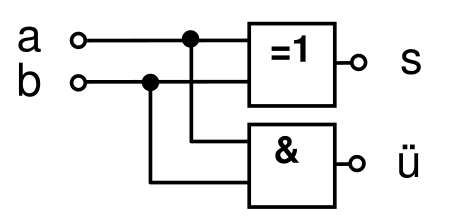
\includegraphics[width=\linewidth]{pictures/halfadder1}
\endminipage\hfill
\minipage{0.32\textwidth}%
  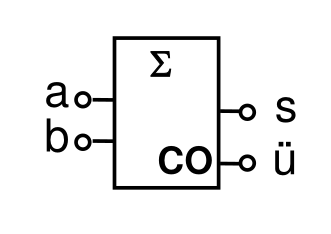
\includegraphics[width=\linewidth]{pictures/halfadder2}
\endminipage
\end{frame}

\subsection{Volladdierer}
\begin{frame}{Mehrstellige Dualzahlen}
\begin{itemize}
	\item Zusätzlicher Eingang für den Übertrag der vorhergehenden Stellen ist nötig
	\begin{table}[]
	\begin{tabular}{ccc|cc}
$a_i$ & $b_i$ & $c_i$ & $s_i$ & $c_{i+1}$ \\ \hline
0 & 0 & 0 & 0 & 0 \\
0 & 1 & 0 & 1 & 0 \\
0 & 1 & 1 & 0 & 1 \\
1 & 0 & 0 & 1 & 0 \\
1 & 0 & 1 & 0 & 1 \\
1 & 1 & 0 & 0 & 1 \\
1 & 1 & 1 & 1 & 1 \\
\end{tabular}
\end{table}
	\item Dies nennt man einen \textcolor{red}{Volladdierer}
\end{itemize}
\end{frame}

\begin{frame}{Gleichungen, Schaltnetz und Schaltsymbol}
\begin{itemize}
	\item Ausgangsgleichungen:
	\begin{align*}
	s_i & = a_i \oplus b_i \oplus c_i \\
	c_{i+1} &= a_i \land c_i \lor b_i \land c_i \lor a_i \land b_i = (a_i \oplus b_i) \land c_i \lor a_i \land b_i
	\end{align*}
\end{itemize}
\minipage{0.45\textwidth}
  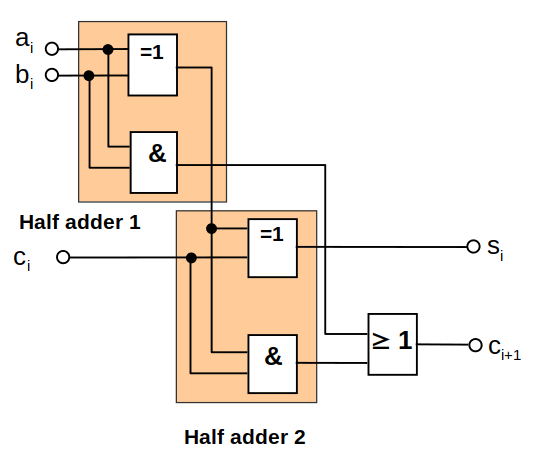
\includegraphics[scale=0.35]{pictures/fulladder1}
\endminipage \hfill
\minipage{0.45\textwidth}%
  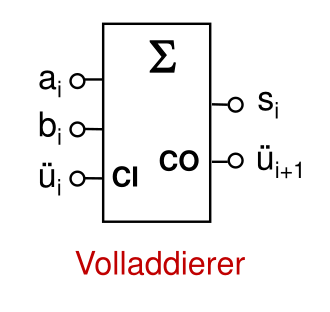
\includegraphics[scale=0.3]{pictures/fulladder2}
\endminipage
\end{frame}

\subsection{Carry-ripple-Addierer}

\begin{frame}{Carry-ripple-Addierer}
\begin{itemize}
	\item Addieren zweier Dualzahlen mit mehreren Stellen
	\item Einfachste Lösung:
	\begin{itemize}
		\item Für jede Stelle einen Volladdierer vorsehen und den Übertrag der Stelle $i$ im Volladdierer der Stelle $i+1$ berücksichtigen
		\item Die Stelle geringster Wertigkeit (LSB, least significant bit) kann mit einem Halbaddierer realisiert werden
	\end{itemize}
\begin{figure}
\center
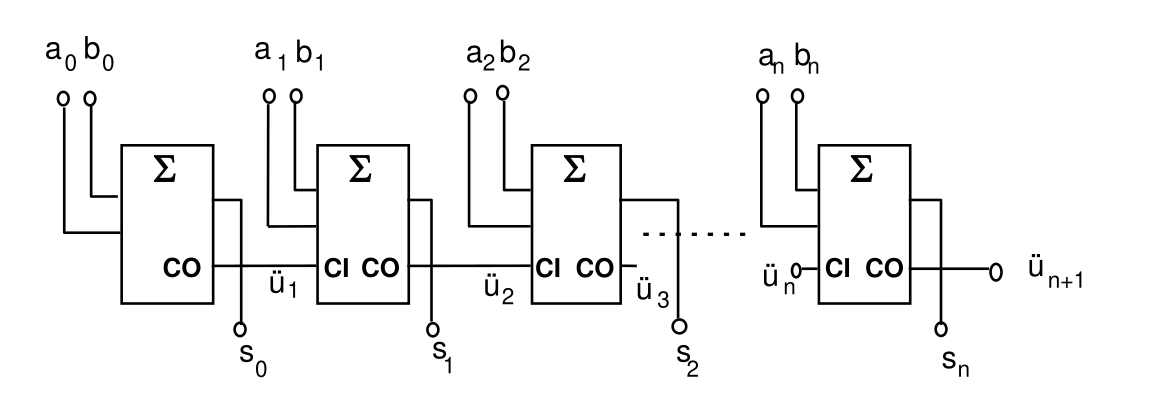
\includegraphics[scale=0.3]{pictures/carry_ripple_adder}
\end{figure}
\end{itemize}
\end{frame}

\begin{frame}{Probleme}
\begin{itemize}
	\item Ergebnis der Addition einer Stelle ist erst dann gültig, wenn der Übertrag aus der vorhergehenden Stelle berechnet ist
	\item Ungünstiger Fall: Das Durchlaufen durch alle Stufen muss abgewartet werden (Carry-ripple-Addierer, to ripple = rieseln)
	\item Die Stabilisierungsdauer ist proportional zur Anzahl der Stellen
	\item Man nennt den Carry-ripple-Addierer auch \textcolor{red}{Asynchroner Parallel-Addierer}, da er bit-parallel addiert, d.h. alle Bits der Operanden gleichzeitig benutzt
\end{itemize}
\end{frame}

\begin{frame}{Carry-lookahead-Addierer}
\begin{itemize}
	\item Um den Nachteil der großen Additionszeit des Carry-ripple-Addierers zu vermeiden:
	\begin{itemize}
		\item \textcolor{red}{Alle Überträge direkt aus den Eingangsvariablen bestimmen (Carry-Lookahead)}
	\end{itemize}
	\item Es gilt:
	\begin{align*}
	c_{i+1}	&= a_i \land b_i (a_i \oplus b_i) \land c_i &= g_i \lor p_i c_i \\
	s_i 	&= (a_i \oplus b_i) \oplus c_i &= p_i \oplus c_i
	\end{align*}
	mit
	\begin{itemize}
		\item $g_i = a_i \land b_i$ (generate carry, erzeuge Übertrag) und
		\item $p_i = (a_i \oplus b_i)$ (propagate carry, leite Übertrag weiter)
	\end{itemize}
	\item $g_i$ und $p_i$ können direkt aus den Eingangsvariablen erzeugt werden
\end{itemize}
\end{frame}

\subsection{Carry-lookahead-Addierer}

\begin{frame}{Berechnung der Überträge aus den Eingangsvariablen}
\begin{itemize}
	\item Die rekursive Berechnung der Übertrage $c_i$ kann aufgelöst werden, indem sukzessive die Ausdrücke für die Berechnung des Übertrags in den vorhergehenden Stellen eingesetzt werden\\
	$\qquad \qquad \qquad c_{i+1} = g_i \lor p_i \land c_i$
	\item Man erhält
	\begin{align*}
	c_1 &= g_0 \lor p_0 \land c_0 \\
	c_2 &= g_1 \lor p_1 \land g_0 \lor p_1 \land p_0 \land c_0\\
	c_3 &= g_2 \lor p_2 \land g_1 \lor p_2 \land p_1 \land g_0 \lor p_2 \land p_1 \land p_0 \land c_0\\
	\ldots & \\
	c_n &= g_{n-1} \lor p_{n-1} \ldots \land c_0
	\end{align*}
	\item Die Additionszeit wird damit weitgehend unabhängig von der Stellenzahl, weil die Berechnung des
Übertrags in allen Stufen sofort (vorausschauend) beginnen kann. Deshalb wird dieser Addierer als \textcolor{red}{Carry-lookahead-Addierer} bezeichnet
\end{itemize}
\end{frame}

\begin{frame}{Schaltbild: 3-Bit-Carry-lookahead-Addierer}
\begin{figure}
\center
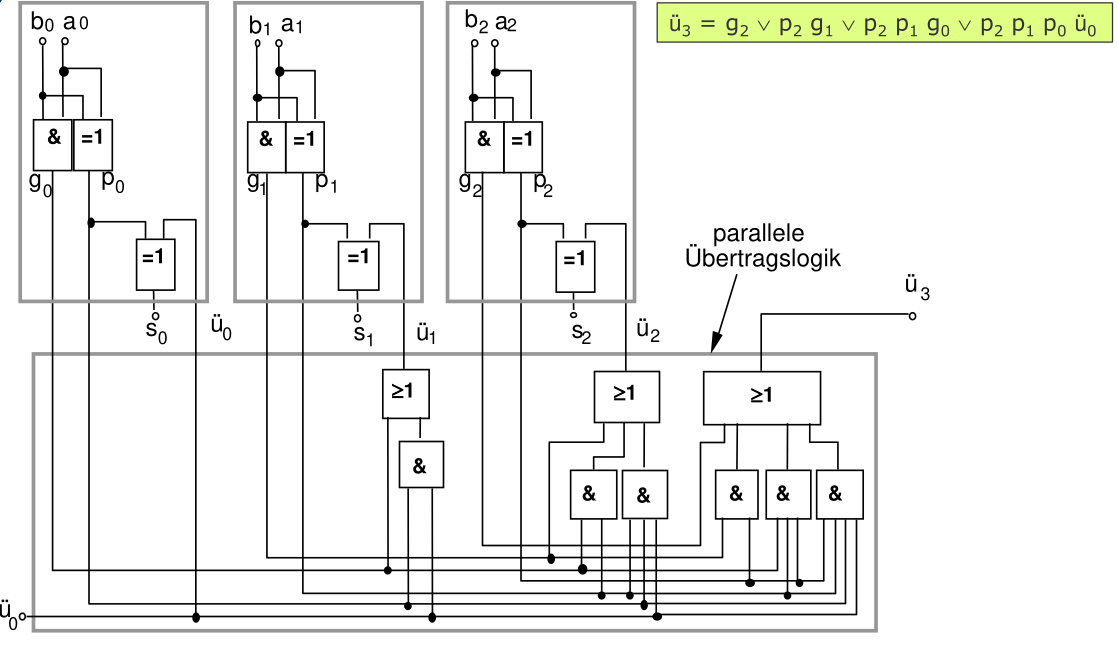
\includegraphics[scale=0.3]{pictures/carry_lookahead_adder}
\end{figure}
\end{frame}

\begin{frame}{Carry-lookahead-Addierer}
\begin{itemize}
	\item Problem:
	\begin{itemize}
		\item Größe des Hardware-Aufwands steigt mit steigender Stellenzahl stark an.
	\end{itemize}
	\item Lösungen:
	\begin{itemize}
		\item kleinere Carry-lookahead-Addierer mit paralleler Übertragserzeugung, die seriell kaskadiert werden
		\item Blocküberträge der kleineren Blöcke parallel verarbeiten
		\item $\Rightarrow$ Hierarchie von Carry-lookahead-Addierern
	\end{itemize}
\end{itemize}
\end{frame}

\begin{frame}{Carry-lookahead-Addierer Kaskadierung}
Kaskadierung zweier 4-Bit Carry-lookahead-Addierer zur Addition von 8-Bit-Zahlen
\begin{figure}
\center 
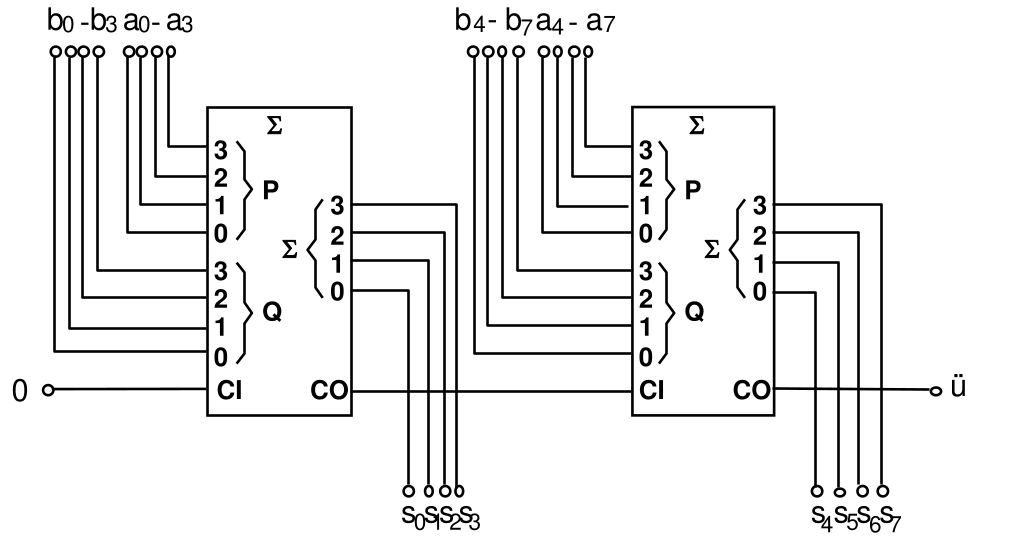
\includegraphics[scale=0.35]{pictures/carry_lookahead_adder2}
\end{figure}
\end{frame}

\section{Subtraktion}
\begin{frame}{Subtraktion}
\begin{itemize}
	\item Subtraktion durch Addition des Zweierkomplements
	\item Zweierkomplement: bit-weise Komplementierung der Zahl und anschließende Addition von 1
	$$
		X - Y = X + (\neg Y + 1) = X + \neg Y + 1
	$$
	\item Man beachte:
	\begin{itemize}
		\item Wir nehmen an, wenn beide Eingabezahlen $X,Y$ im Zweierkomplement-Form gegeben sind
		\item $\to$ Am Ausgang entsteht wieder eine Zahl in Zweierkomplement-Form
	\end{itemize}
\end{itemize}
\end{frame}

\begin{frame}{Subtraktion}
\begin{itemize}
	\item Die beiden Additionen können mit einem Addierer vorgenommen werden, indem man den Übertragseingang ausnutzt
\end{itemize}
\begin{figure}
\center
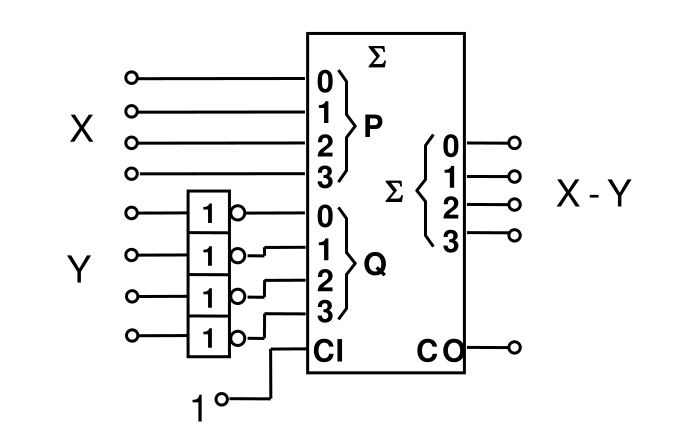
\includegraphics[scale=0.4]{pictures/sub_complement}
\caption{Subtraktion von Zweierkomplementzahlen}
\end{figure}
\end{frame}

\begin{frame}{Sonderfälle}
\minipage{0.68\textwidth}
  \begin{itemize}
	\item Bei der Addition lassen sich 3 Sonderfälle unterscheiden
	\begin{enumerate}
		\item Beide Summanden sind positiv
		\begin{itemize}
			\item die Vorzeichenbits beider Zahlen sind 0
			\item das Ergebnis muss positiv sein
			\item Das Ergebnis ist nur dann korrekt, wenn sein Vorzeichenbit gleich 0 ist, ansonsten wurde der Zahlenbereich überschritten
			\item Man kann sich diese Situation anhand des Zahlenkreises klarmachen
		\end{itemize}
	\end{enumerate}
\end{itemize}
\endminipage\hfill
\minipage{0.28\textwidth}%
  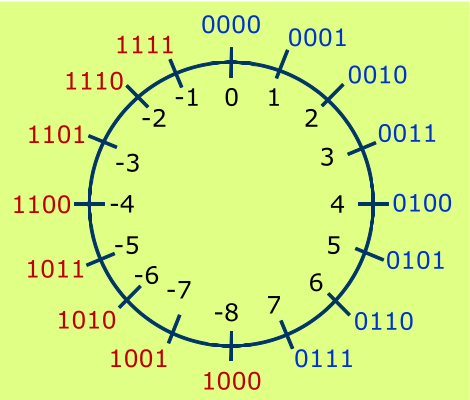
\includegraphics[scale=0.3]{pictures/sub1}
\endminipage
\begin{figure}
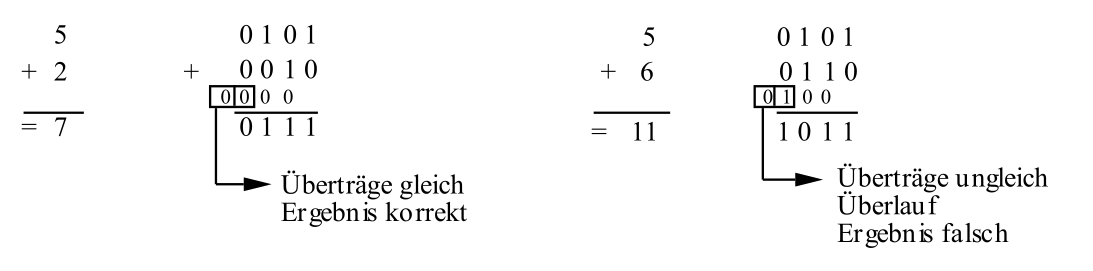
\includegraphics[scale=0.27]{pictures/sub2}
\end{figure}
\end{frame}

\begin{frame}{Sonderfall 2}
\minipage{0.68\textwidth}
	\begin{enumerate} \setcounter{enumi}{1}
		\item Beide Summanden sind negativ
		\begin{itemize}
			\item Die Vorzeichenbits beider Zahlen haben den Wert 1
			\item Das Ergebnis muss negativ sein
			\item Das Ergebnis ist nur dann korrekt, wenn das Vorzeichenbit des Ergebnisses 1 ist
			\item Die beiden vordersten Überträge müssen den gleichen Wert haben
		\end{itemize}
	\end{enumerate}
\endminipage\hfill
\minipage{0.28\textwidth}%
  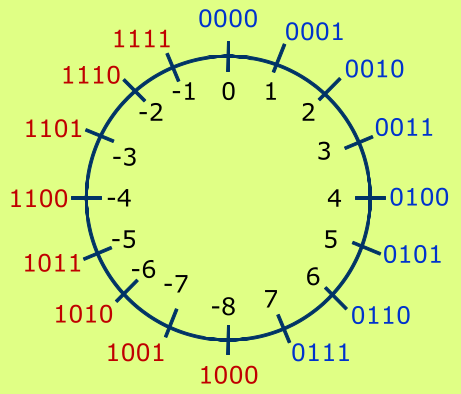
\includegraphics[scale=0.3]{pictures/sub3}
\endminipage
\begin{figure}
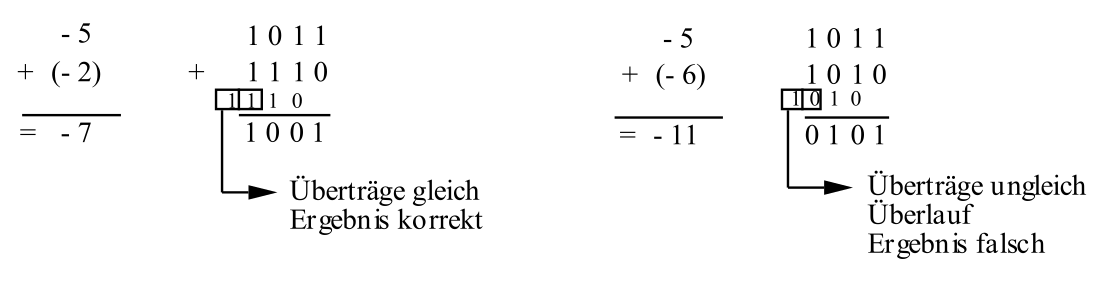
\includegraphics[scale=0.27]{pictures/sub4}
\end{figure}
\end{frame}

\begin{frame}{Sonderfall 3}
\minipage{0.68\textwidth}
	\begin{enumerate} \setcounter{enumi}{2}
		\item Beide Summanden haben unterschiedliche Vorzeichen
		\begin{itemize}
			\item Das Ergebnis ist auf jeden Fall korrekt, das Vorzeichen hängt davon ab, ob Subtrahend oder Minuend betragsmäßig größer ist
			\item Der Übertrag aus der vordersten Stelle ist zu streichen
		\end{itemize}
	\end{enumerate}
\endminipage\hfill
\minipage{0.28\textwidth}%
  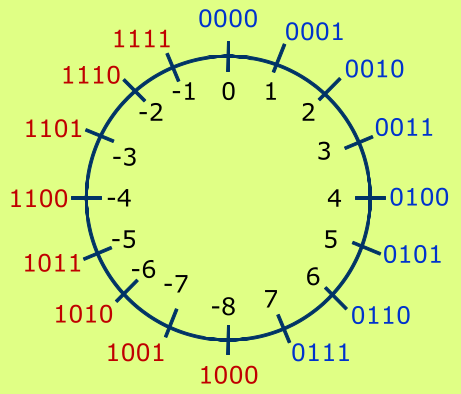
\includegraphics[scale=0.3]{pictures/sub3}
\endminipage
\begin{figure}
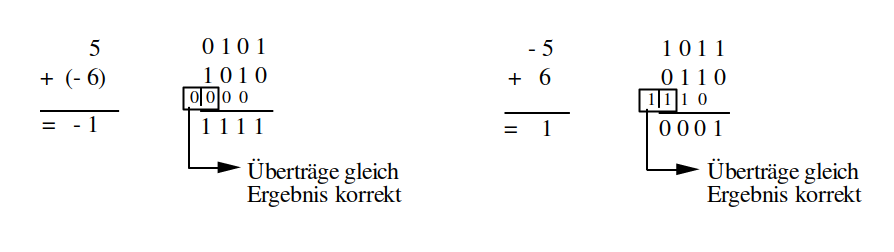
\includegraphics[scale=0.32]{pictures/sub5}
\end{figure}
\end{frame}

\subsection{Überlauferkennung}

\begin{frame}{Überlauferkennung}
\begin{itemize}
	\item Allgemeine Überlauferkennung bei dualer Addition:
	\begin{itemize}
		\item korrekte Addition: beide Überträge sind gleich
		\item Überlauf: beide Überträge sind ungleich
	\end{itemize}
	\item Realisierung z.B. durch ein Antivalenzgatter (XOR)
\end{itemize}
\end{frame}

\section{Gleitkomma-Addition}

\begin{frame}{Zusatzbetrachtung: Gleitkomma-Addition}
	\begin{itemize}
		\item Addition von zwei Gleitkommazahlen $a_1$ und $a_2$
		$$
			a_1 = s_1 \cdot b^{e_1} \qquad \qquad a_2 = s_2 \cdot b^{e_2}
		$$
		\item Beispiel:
		\begin{itemize}
			\item $a_1 = 3,21 \cdot 10^2$
			\item $a_2 = 8,43 \cdot 10^{-1}$
		\end{itemize}
		\item Gerechnet wird mit zwei zusätzlichen Stellen in der Mantisse (Guard und Round) sowie dem Sticky-Bit
	\end{itemize}
	\begin{figure}
	\center
	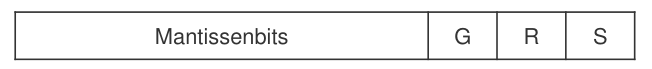
\includegraphics[scale=0.3]{pictures/mantisse}
	\end{figure}
\end{frame}

\begin{frame}{Gleitkomma-Addition}
\begin{enumerate}
	\item Exponentenangleichung
	\begin{itemize}
		\item Gleitkommazahlen können nur addiert werden, wenn die Exponenten gleich sind
		\item Schritt 1: Wenn $e_1 < e_2$, dann vertausche die Operanden, so dass gilt: $d = e_1 - e_2 \geq 0$
		\item Schritt 2: Verschiebe die Mantisse $s_2$ um $d$ Stellen nach rechts
		\begin{itemize}
			\item Wenn $d > 2$, setze das Sticky Bit, falls die $d-2$ herausgeschobenen Stellen einen Wert $\neq 0$ ergeben
		\end{itemize}
		\item Im Beispiel: $d = 2 - (-1) = 3$
		\begin{align*}
		3,2100 & \cdot 10^2\\
		0,0084 & \cdot 10^2 \qquad \text{Sticky-Bit gesetzt, da die 3 aus 8,43 herausgeschoben wird}
		\end{align*}
	\end{itemize}
\end{enumerate}
\end{frame}

\begin{frame}{Gleitkomma-Addition}
\begin{enumerate} \setcounter{enumi}{1}
	\item Mantissenaddition
	\begin{itemize}
		\item Addiere die beiden Mantissen
		\item Im Beispiel:
		\begin{align*}
		3,2100 & \cdot 10^2 \\
		0,0084 & \cdot 10^2 \\ \cline{1-2}
		3,2184 & \cdot 10^2
		\end{align*}
	\end{itemize}
	\item Normalisierung
	\begin{itemize}
		\item Normalisiere die entstandene Summe durch Verschieben der Mantisse und Korrektur des Exponenten
	\end{itemize}
\end{enumerate}
\end{frame}

\begin{frame}{Gleitkomma-Addition}
\begin{enumerate} \setcounter{enumi}{3}
	\item Rundung
	\begin{itemize}
		\item Runde unter Berücksichtigung der Stellen g, r und des Sticky-Bits, sowie der gegebenen Rundungsart (meist \enquote{round-to-even})
		\item Im Beispiel:
		\begin{align*}
		3,2100 & \cdot 10^2 \\
		0,0084 & \cdot 10^2 \\ \cline{1-2}
		3,2184 & \cdot 10^2
		\end{align*}
	\end{itemize}
	\item Ergebnis wird gerundet zu: $3,22 \cdot 10^2$
\end{enumerate}
\end{frame}

\begin{frame}{Beispiel 1: $32 - 2.25 = 30$ mit $4$ Genauigkeit 4, $q = 2$}
\minipage{0.48\textwidth}
  $ 1.000 \cdot 2^5 - 1.001 \cdot 2^1$\\
  Unendliche Genauigkeit
  \begin{align*}
  & 1.000 & 0000 & \cdot 2^5  & \\ 
 -& 0.000 & 1001 & \cdot 2^5 & \text{anpassen} \\ \cline{2-3}
  & 0.111 & 0111 & \cdot 2^5 & \text{prez. 29.75}\\
  & 1.110 & 1110 & \cdot 2^4 & \text{norm.} \\
  & 1.111  &    & \cdot 2^4 & \text{runden}\\
  \end{align*}
\endminipage \hfill
\minipage{0.48\textwidth}%
   Nutzung von \textcolor{blue}{G}uard, \textcolor{green}{R}ound, \textcolor{red}{S}ticky Bits\\
   Plus 4 Stellen Genauigkeit
  \begin{align*}
  & \overbrace{1.000} & 000 & \cdot 2^5  & \\ 
 -& 0.000 & \textcolor{blue}{1}\textcolor{green}{0}\textcolor{red}{1} & \cdot 2^5 &\\ \cline{2-3}
  & 0.111 & \textcolor{blue}{0}\textcolor{green}{1}\textcolor{red}{1} & \cdot 2^5 &\\
  & 1.11 \textcolor{blue}{0} & \textcolor{green}{1}\textcolor{red}{1} & \cdot 2^4 & \text{norm.} \\
  & 1.111 &     & \cdot 2^4 & \text{runden}\\
  \end{align*}
\endminipage
\end{frame}

\begin{frame}{MIPS R10000 Floating-point Unit}
\begin{figure}
\center
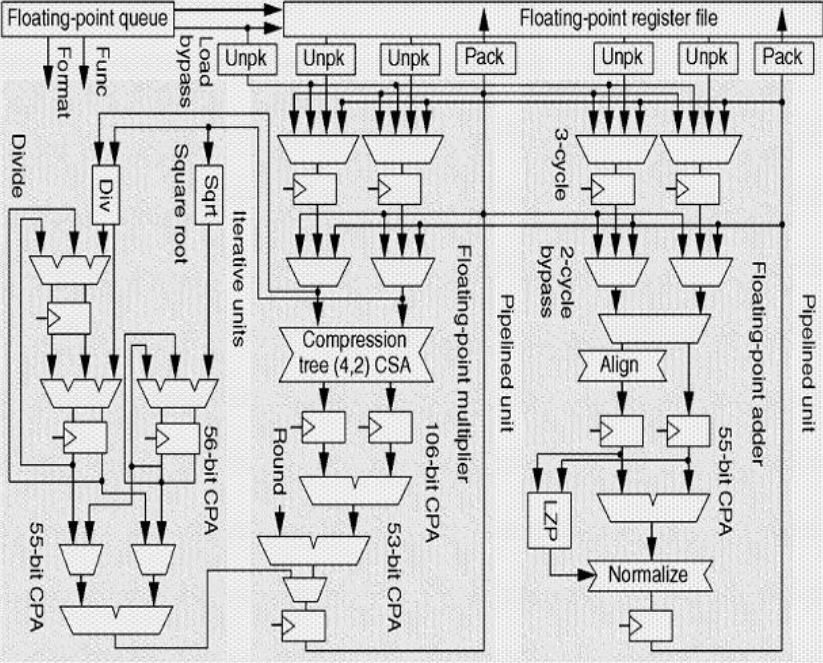
\includegraphics[scale=0.3]{pictures/mips1000_fpu}
\end{figure}
\end{frame}

\section{Arithmetisch-logische Einheit}

\begin{frame}{Arithmetisch-logische Einheit}
\begin{itemize}
	\item Arithmetisch-logische Einheit (ALU, arithmetic logic unit):
	\begin{itemize}
		\item Rechenwerk, der funktionale Kern eines Digitalrechners zur Durchführung logischer und arithmetischer Verknüpfungen
	\end{itemize}
	\item Eingangsdaten der ALU:
	\begin{itemize}
		\item Daten und Steuersignalen vom Prozessor
	\end{itemize}
	\item Ausgangsdaten der ALU:
	\begin{itemize}
		\item Ergebnisse und Statussignale an den Prozessor
	\end{itemize}
	\item Oft können die in einen Prozessor integrierten ALUs nur Festkommazahlen verarbeiten. Die Gleitkommaoperationen werden dann entweder von einer Gleitkommaeinheit ausgeführt oder per Software in eine Folge von Festkommabefehlen umgewandelt
\end{itemize}
\end{frame}

\begin{frame}{Schema einer einfachen ALU}
\begin{figure}
\center
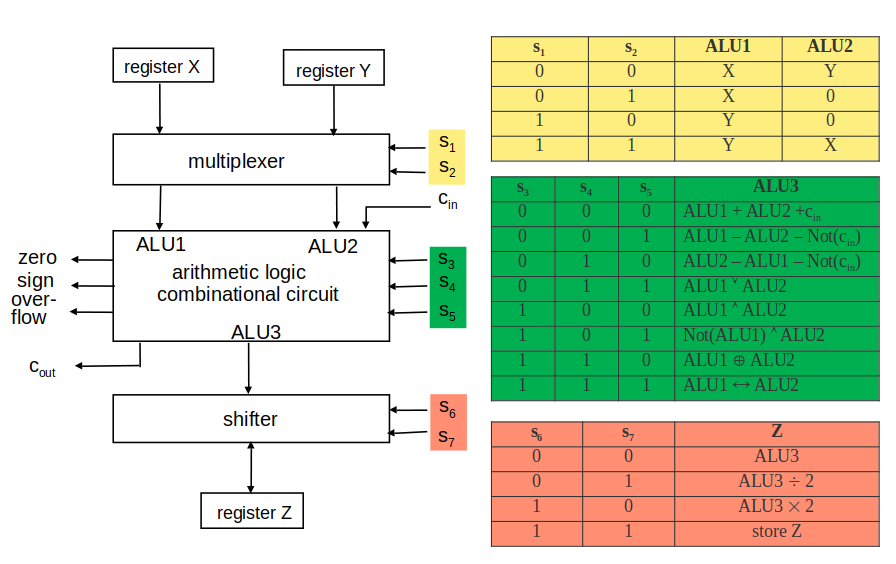
\includegraphics[scale=0.4]{pictures/simple_alu}
\end{figure}
\end{frame}

\begin{frame}{Bestandteile der ALU}
\begin{itemize}
	\item Registersatz
	\item Multiplexerschaltnetz
	\item Arithmetisch logisches Schaltnetz zur Durchführung arithmetisch logischer Operationen 
	\item Schiebeschaltnetz
	\item Eingänge:
	\begin{itemize}
		\item Datenworte $X$ und $Y4$
		\item Steuersignale $s_1 \ldots s_7$ zur Festlegung der ALU-Operation
	\end{itemize}
	\item Ausgänge:
	\begin{itemize}
		\item Statussignale zero, sign und overflow
		\item Hiermit kann das Steuerwerk bestimmte ALU-Zustände erkennen und darauf entsprechend reagieren
	\end{itemize}
\end{itemize}
\end{frame}

\begin{frame}{Beispiele}
\begin{itemize}
	\item Einerkomplement von $Y$ um ein Bit nach links verschoben in $Z$ ablegen
	\begin{itemize}
		\item Steuersignale: $s_1 \ldots s_7 = 10 111 10$
		\item 10 : $ALU1 = Y$
		\item 111: $ALU3 = ALU1 \leftrightarrow ALU2$
		\item 10: $Z = ALU3 \cdot 2$
	\end{itemize}
	\item Ist $X > Y$ ?
	\begin{itemize}
		\item Statussignal \enquote{sign} bei der Operation $Y - X$
		\item Steuersignale: $s_1 \ldots s7 = 00 010 00$ und $c_{in} = 1$
		\begin{itemize}
			\item 00 : $ALU1 = X$ und $ALU2 = Y$
			\item 010: $ALU3 = ALU2 - ALU1 - not(c_{in})$
			\item 00 : $Z = ALU3$
		\end{itemize}
	\end{itemize}
\end{itemize}
\end{frame}

\section*{Quellen}
\appendix
\begin{frame}[allowframebreaks]
  \frametitle<presentation>{Quellen}
\printbibliography
\end{frame}
\end{document}